\documentclass[10 pt,usenames,dvipsnames, oneside]{article}
\usepackage{../../../modelo-ensino-medio}



\begin{document}

\begin{center}
  \begin{minipage}[l]{3cm}
\includegraphics[width=2cm]{logo}    
\end{minipage}\hfill
\begin{minipage}[r]{.8\textwidth}
 {\Large \scshape Atividade: A maratona}  
\end{minipage}
\end{center}
\vspace{.2cm}

\ifdefined\prof
%Habilidades da BNCC
\begin{objetivos}
\item \textbf{EM13MAT316} Estudar o efeito de uma transformação simples numa
distribuição de dados: adição (posição) e multiplicação (escala).
\item \textbf{EM13MAT408} Construir e interpretar tabelas e gráficos de frequências, com base em dados obtidos em pesquisas por amostras estatísticas, incluindo ou não o uso de softwares que interrelacionem estatística, geometria e álgebra.
\end{objetivos}

%Caixa do Para o Professor
\begin{goals}
%Objetivos específicos
\begin{enumerate}
\item Identificar a posição da média e dos quartis no gráfico da
distribuição de frequências (histograma).
\item  Apresentar representação gráfica alternativa ao histograma: box-plot
sem a sinalização de valores discrepantes.
\end{enumerate}

\tcblower

%Orientações e sugestões
Nesta atividade serão apresentados conjuntos diferentes de dados envolvendo tempos para completar maratonas. Os dados estão disponíveis neste \href{https://www.geogebra.org/m/ZhqKD9Nz}{link}. Serão fornecidos os totais para que o cálculo das médias envolva apenas uma divisão e possa ser feito com uma calculadora simples. Pretende-se levar o aluno a perceber que na presença de forte assimetria (histograma alongado à direita ou à esquerda), a média pode não ser a medida mais adequada para representar o conjunto e, com isso, motivar a definição de mediana.

É importante discutir as perguntas na caixa Para refletir em sala de aula com o intuito de que os estudantes percebam a necessidade de tratar previamente dados de determinada natureza antes de usá-los numericamente, como é o caso do tempo considerado em unidades distintas (hora:minuto:segundo).

Na sequência se inclui a tabela com a respectiva conversão para minutos em números decimais de modo a simplificar os cálculos na atividade, mas deve-se deduzir com os estudantes como calcular a conversão.

Expressão utilizada para calcular o resultado em minutos decimais (minutos$_{10}$):
\begin{equation*}
\text{minutos}_{10}=\text{Horas}\cdot60+\text{Minutos}+\frac{\text{Segundos}}{60}
\end{equation*}
É importante comentar com os estudantes a diferença observada entre a média e a mediana e que esta se deve a uma forte assimetria na distribuição dos dados, representada pela forma de um histograma alongado para à esquerda com frequências pequenas, tornando a média inferior à mediana.

Sugere-se como atividade interdisciplinar, a realização de corridas com os estudantes na Educação Física, medindo os tempos totais, calculando a velocidade média do percurso e comparando com a velocidade média do primeiro e centésimo lugares da maratona. Recomenda-se explicitar o vínculo com a Física para o cálculo e a interpretação da velocidade média, assim como a colocação de questões críticas que facilitem a interpretação dos resultados, por exemplo, é possível manter essa velocidade média durante quase $3$ horas (tempo médio da maratona de mulheres)?

\end{goals}

\bigskip
\begin{center}
{\large \scshape Atividade}
\end{center}
\fi

A maratona é uma prova de atletismo que consiste em correr uma distância de $42.195$ km. Pelas suas características, este tipo de prova é realizada nas ruas de uma grande cidade ou na estrada. As principais cidades do mundo realizam um destes eventos anualmente, recebendo milhares de atletas profissionais e amadores que encaram o desafio e almejam finalizar a corrida ou melhorar o próprio tempo do passado.

Uma das mais famosas é a Maratona da Cidade de Nova Iorque, nos Estados Unidos. Veja na figura \hyperref[\detokenize{PE104-0:fig-maratona-ny}]{Corredores participando da Maratona de Nova York, Wikipedia} realização de uma maratona em Nova Iorque. Com mais de 50.000 participantes cada ano, é um dos principais eventos do atletismo mundial, junto com as maratonas de Chicago, Londres, Boston, Berlim e Tóquio.

\begin{figure}[H]
\centering

\includegraphics[width=200bp]{{New_York_marathon_Verrazano_bridge}.jpg}
\caption{Corredores participando da Maratona de \textit{Nova York}, 
\href{https://commons.wikimedia.org/wiki/File:New\_York\_marathon\_Verrazano\_bridge.jpg}{Wikipedia}}
\label{\detokenize{PE104-0:fig-maratona-ny}}
\label{\detokenize{PE104-0:id11}}
\end{figure}

Os resultados do evento são divididos nas categorias de homens e mulheres, além disso, no evento participam cadeirantes e pessoas usando triciclos de mão (\textit{handcycle}), categorias cujos resultados são premiados e publicados separadamente. Qual das categorias você acha que terá os melhores resultados na maratona? Em quanto tempo você acha que uma pessoa percorre os $42.195$ km? O que você acha ser mais rápido: correr em cadeira de rodas ou em triciclo de mão?

\phantomsection\label{\detokenize{PE104-0:handcycle}}
\begin{figure}[H]
\centering
\includegraphics[width=200bp]{{Handcycle_in_Richmond_Park_-_geograph.org.uk_-_1315077}.jpg}
\label{\detokenize{PE104-0:handcycle}}
\end{figure}

A seguir analisaremos os tempos de corrida das 100 melhores atletas na categoria de Mulheres da Maratona de Nova York do ano 2017, dados disponíveis no \href{http://results.nyrr.org/event/M2017/finishers}{site oficial da competição}.

Observe no quadro a seguir, que os tempos já estão ordenados do menor para o maior e que para identificar o tempo da quadragésima sétima chegada, basta tomar a interseção da linha $7$ com a coluna $+40$ para obter o tempo $2:55:36$, ou seja, duas horas $55$ minutos e $36$ segundos.



\begin{table}[H]
\centering
\caption{100 melhores tempos de finalização da Maratona de Nova Iorque 2017 para mulheres (hora:minuto:segundo)}
\setlength\tabcolsep{2.5pt}
\label{\detokenize{PE104-0:id12}}
\begin{tabular}{|c|r|r|r|r|r|r|r|r|r|r|}
\hline
\tcolor{}& \tcolor{+0} & \tcolor{+10} & \tcolor{+20} & \tcolor{+30} & \tcolor{+40} & \tcolor{+50} & \tcolor{+60} & \tcolor{+70} & \tcolor{+80} & \tcolor{+90} \\
\hline
1 & 2:26:53 & 2:32:01 & 2:42:52 & 2:49:44 & 2:53:59 & 2:56:58 & 2:58:35 & 2:59:36 & 3:01:24 & 3:03:43 \\
\hline
2 & 2:27:54 & 2:32:09 & 2:44:26 & 2:49:59 & 2:54:42 & 2:57:05 & 2:58:36 & 2:59:41 & 3:01:26 & 3:03:46 \\
\hline
3 & 2:28:08 & 2:33:18 & 2:44:48 & 2:50:04 & 2:54:52 & 2:57:10 & 2:58:50 & 2:59:43 & 3:01:28 & 3:04:02 \\
\hline
4 & 2:29:36 & 2:34:10 & 2:45:20 & 2:50:05 & 2:55:04 & 2:57:40 & 2:58:52 & 2:59:46 & 3:01:44 & 3:04:04 \\
\hline
5 & 2:29:39 & 2:34:23 & 2:45:52 & 2:51:11 & 2:55:25 & 2:57:49 & 2:58:56 & 2:59:51 & 3:02:09 & 3:04:17 \\
\hline
6 & 2:29:39 & 2:36:38 & 2:46:45 & 2:53:01 & 2:55:34 & 2:57:49 & 2:59:01 & 2:59:56 & 3:02:15 & 3:04:26 \\
\hline
7 & 2:29:41 & 2:37:22 & 2:47:04 & 2:53:02 & 2:55:36 & 2:57:50 & 2:59:03 & 3:00:02 & 3:02:39 & 3:04:42 \\
\hline
8 & 2:29:56 & 2:37:33 & 2:47:30 & 2:53:02 & 2:55:39 & 2:58:08 & 2:59:10 & 3:00:05 & 3:02:41 & 3:04:49 \\
\hline
9 & 2:31:21 & 2:39:01 & 2:47:35 & 2:53:19 & 2:56:47 & 2:58:23 & 2:59:16 & 3:00:49 & 3:02:56 & 3:04:58 \\
\hline
10 & 2:31:44 & 2:40:09 & 2:49:37 & 2:53:38 & 2:56:57 & 2:58:26 & 2:59:23 & 3:01:18 & 3:03:32 & 3:05:09 \\
\hline
\end{tabular}
\end{table}

Para calcular a média destes dados é conveniente reduzi-los a uma única unidade de medida, pois, caso contrário, seria necessário calcular três médias e, ainda fazer conversões apropriadas para obter a resposta em hora:minuto:segundo. Convertendo todos os tempos para minutos, obtemos o seguinte quadro de tempos arredondados para duas casas decimais.

\begin{table}[H]
\centering
\setlength\tabcolsep{3.5pt}
\begin{tabular}{|c|r|r|r|r|r|r|r|r|r|r|}
\hline
\tcolor{}& \tcolor{+0} & \tcolor{+10} & \tcolor{+20} & \tcolor{+30} & \tcolor{+40} & \tcolor{+50} & \tcolor{+60} & \tcolor{+70} & \tcolor{+80} & \tcolor{+90} \\
\hline
1 & 146,88 & 152,02 & 162,87 & 169,73 & 173,98 & 176,97 & 178,58 & 179,60 & 181,40 & 183,72 \\
\hline
2 & 147,90 & 152,15 & 164,43 & 169,98 & 174,70 & 177,08 & 178,60 & 179,68 & 181,43 & 183,77 \\ 
\hline
3 & 148,13 & 153,30 & 164,80 & 170,07 & 174,87 & 177,17 & 178,83 & 179,72 & 181,47 & 184,03 \\
\hline
4 & 149,60 & 154,17 & 165,33 & 170,08 & 175,07 & 177,67 & 178,87 & 179,77 & 181,73 & 184,07 \\
\hline
5 & 149,65 & 154,38 & 165,87 & 171,18 & 175,42 & 177,82 & 178,93 & 179,85 & 182,15 & 184,28 \\
\hline
6 & 149,65 & 156,63 & 166,75 & 173,02 & 175,57 & 177,82 & 179,02 & 179,93 & 182,25 & 184,43 \\
\hline
7 & 149,68 & 157,37 & 167,07 & 173,03 & 175,60 & 177,83 & 179,05 & 180,03 & 182,65 & 184,70 \\
\hline
8 & 149,93 & 157,55 & 167,50 & 173,03 & 175,65 & 178,13 & 179,17 & 180,08 & 182,68 & 184,82 \\
\hline
9 & 151,35 & 159,02 & 167,58 & 173,32 & 176,78 & 178,38 & 179,27 & 180,82 & 182,93 & 184,97 \\
\hline
10 & 151,73 & 160,15 & 169,62 & 173,63 & 176,95 & 178,43 & 179,38 & 181,30 & 183,53 & 185,15 \\
\hline
\end{tabular}
\end{table}

\begin{enumerate}
\item {} 
Construa um histograma dos dados convertidos para horas, completando a \hyperref[tabela-maratona3]{tabela \ref{tabela-maratona3}}, que indica os intervalos de classe (fechados no limite inferior e abertos no limite superior).

\begin{table}[H]
\centering
\begin{tabular}{|l|c|}
\hline
\tcolor{Intervalo} & \tcolor{Frequência} \\
\hline
$[146{,}0 ; 150{,}0 [$ & \\
\hline
$[150{,}0 ; 154{,}0 [$ & \\
\hline
$[154{,}0 ; 158{,}0 [$ & \\
\hline
$[158{,}0 ; 162{,}0 [$ & \\
\hline
$[162{,}0 ; 166{,}0 [$ & \\
\hline
$[166{,}0 ; 170{,}0 [$ & \\
\hline
$[170{,}0 ; 174{,}0 [$ & \\
\hline
$[174{,}0 ; 178{,}0 [$ & \\
\hline
$[178{,}0 ; 182{,}0 [$ & \\
\hline
$[182{,}0 ; 186{,}0 [$ & \\
\hline
\end{tabular}
\caption{Intervalos de classes}
\label{tabela-maratona3}
\end{table}
% \begin{figure}[H]
% \centering
% \capstart

% \begin{tikzpicture}[scale=.8, every node/.style={scale=.8}]
% \begin{scope}[x=500, y = 7]
% 	\foreach \ye in {0,2,...,30}{
% 		\draw [help lines, lightgray] (2.4480,\ye) -- (3.0860,\ye);
% 		\draw (2.4480,\ye) -- (2.435,\ye);
% 		\node [left] at (2.435,\ye) {\ye} ;
% 	}
% 	\foreach \xe in {2.4480,2.5118,2.5756,2.6394,2.7032,2.7670,2.8308,2.8946,2.9584,3.0222,3.0860}{
% 		\draw [help lines, lightgray] (\xe,0) -- (\xe,30);
% 		\draw (\xe,0) -- (\xe,-1);
% 		\node [right,rotate=-90] at (\xe,-1) {\xe} ;
% 	}
% 	\draw (2.4480,30) -- (2.4480,0) -- (3.0860,0);
% %	\filldraw[fill=destacado] (5.5,0) -- (5.4,-3) -- (5.6,-3) -- cycle;
% %	\node [below] at (5.5,-3) {média};
% \end{scope}

% \end{tikzpicture}\caption{Eixos para a construção do histograma}\label{\detokenize{PE104-0:hist-maratona-mulheres}}\label{\detokenize{PE104-0:id15}}\end{figure}

\item {} 
Calcule o tempo médio dos 100 melhores tempos das corredoras, sabendo que a soma dos tempos é $17.191{,}66$ minutos. Localize o valor encontrado no eixo horizontal do histograma. Em que posição ficaria uma corredora cujo tempo no qual completou a maratona é igual ao tempo médio calculado neste item?


\item {} 
Trace linhas verticais no histograma de modo a separar as classificações em 4 grupos: uma linha vertical que identifica o 25$^{\circ}$ lugar, separando os 25 primeiros colocados dos demais; outra, que identifica a 50$^{\text{a}}$ classificação e, por fim, uma que marca o 75$^{\circ}$ tempo na classificação geral.

As marcações dos tempos das 25$^{\text{a}}$, 50$^{\text{a}}$ e 75$^{\text{a}}$ posições neste conjunto de 100 observações são chamadas de quartis da distribuição, este conceito será formalizado adiante.

\item {} 
Calcule os comprimentos dos intervalos de tempo determinados pela proposta de divisão no item \titem{d)} e compare-os.

\begin{table}[H]
\centering
\begin{tabular}{|c|c|}
\hline
\tcolor{Intervalo} & \tcolor{Comprimento} \\
\hline
1$^{\circ}$ a 25$^{\circ}$ & \\
\hline
25$^{\circ}$ a 50$^{\circ}$ & \\
\hline
50$^{\circ}$ a 75$^{\circ}$ & \\
\hline
75$^{\circ}$ a 100$^{\circ}$ & \\
\hline
\end{tabular}
\end{table}

Observa-se que os comprimentos dos intervalos são bem diferentes, sendo maiores no início e mais estreitos no final.

Observe que apesar das diferenças de comprimento desses intervalos, cada um deles corresponde a cerca de 25 tempos.

\item {} 
O valor obtido para o tempo médio coincide com alguma das outras marcas feitas no histograma?

\item {} 
Observe que o tempo médio dos 100 melhores tempos para mulheres e o tempo da corredora que chegou em 50\super{o}. lugar são diferentes. Qual deles você escolheria como medida resumo destes dados? Por quê?

\item Que características da distribuição dos 100 melhores tempos para mulheres podem ser destacadas, analisando-se o histograma construído?

(Construção de boxplot simplificado) Considerando os valores mínimo ($146{,}88$ min.) e máximo ($185{,}15$ min.), trace uma reta (vertical ou horizontal), incluindo esse intervalo de variação. Por exemplo, de $146$ a $186$.
\begin{figure}[H]
\centering


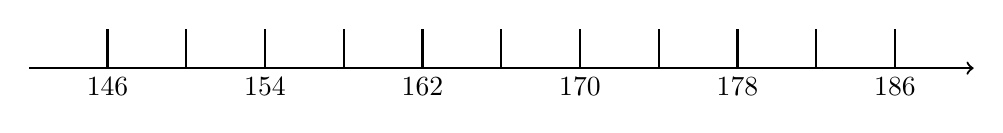
\begin{tikzpicture}
\draw [->,thick] (0,0) -- (12,0);
\foreach \x in {1,...,11} \draw [thick] (\x,0) -- (\x,.5);
\foreach \x/\y in {1/146,3/154,5/162,7/170,9/178,11/186} \node [below] at (\x,0) {$\y$};
\end{tikzpicture}
\caption{Sugestão de escala para a construção do boxplot dos 100 melhores tempos (em minutos) para a categoria mulheres}
\label{}
\end{figure}

Em seguida, trace um retângulo, cujas bases estão nas posições referentes aos 25º e 75º tempos de chegada, cortando o retângulo por um segmento na posição referente ao 50º tempo de chegada. Para terminar a construção, trace um segmento, partindo do ponto médio da parte inferior até o valor mínimo e repita para o ponto médio da parte superior até o valor máximo.

A figura obtida é conhecida como boxplot (gráfico-caixa) do 100 melhores tempos sem a sinalização de valores discrepantes.

O boxplot é uma representação gráfica de dados quantitativos alternativa ao histograma. Esse gráfico é útil na comparação do comportamento de uma variável, considerando diferentes grupos, por exemplo, 100 melhores tempos de chegada entre homens e mulheres.
\end{enumerate}

\ifdefined\prof
\begin{solucao}

\begin{enumerate}
\item A tabela com as frequências por intervalo e o histograma ficam de seguinte forma:

\begin{minipage}{.4\linewidth}
\begin{table}[H]
\centering
\setlength\tabcolsep{2.5pt}
\begin{tabular}{|l|c|}
\hline
\tcolor{Intervalo} & \tcolor{Frequência} \\
\hline
$[146{,}0 ; 150{,}0 [$ & $8$ \\
\hline
$[150{,}0 ; 154{,}0 [$ & $5$ \\
\hline
$[154{,}0 ; 158{,}0 [$ & $5$ \\
\hline
$[158{,}0 ; 162{,}0 [$ & $2$ \\
\hline
$[162{,}0 ; 166{,}0 [$ & $5$ \\
\hline
$[166{,}0 ; 170{,}0 [$ & $7$ \\
\hline
$[170{,}0 ; 174{,}0 [$ & $9$ \\
\hline
$[174{,}0 ; 178{,}0 [$ & $16$ \\
\hline
$[178{,}0 ; 182{,}0 [$ & $27$ \\
\hline
$[182{,}0 ; 186{,}0 [$ & $16$ \\
\hline
\end{tabular}
\caption{Guia para o cálculo de frequências do histograma}

\end{table}
\end{minipage}
\begin{minipage}{.59\linewidth}
\begin{figure}[H]
\centering

\includegraphics[width=\linewidth]{Histograma_mulheres_resposta_1b.png}
\end{figure}
\end{minipage}
\item O tempo médio das primeiras $100$ corredoras é de aproximadamente $171{,}92$ minutos. Uma corredora com esse tempo teria ficado na entre a 35\super{a} e 36\super{a} posição.
\item Para ficar entre os primeiros 25 lugares, uma corredora teria que terminar a corrida em até 165,87 minutos. Já para ficar nas primeiras 50, precisaria terminar o percurso em 176,95 minutos ou menos. Finalmente, para ficar entre as primeiras 75, seu tempo teria que ser menor ou igual a 179,85 minutos.
\begin{figure}[H]
\centering

\includegraphics[width=.6\linewidth]{Histograma_mulheres_resposta_1c.png}
\caption{Histograma dos tempos da categoria de mulheres na Maratona de NY mostrando os quartis, a mediana e a média}
\label{}
\end{figure}

\item Os comprimentos dos intervalos são dados por:
\begin{table}[H]
\centering
\begin{tabular}{|c|c|}
\hline
\tcolor{Intervalo} & \tcolor{Comprimento} \\
\hline
1$^{\circ}$ a 25$^{\circ}$ & $18{,}99$ \\
\hline
25$^{\circ}$ a 50$^{\circ}$ & $11{,}08$ \\
\hline
50$^{\circ}$ a 75$^{\circ}$ & $2{,}90$ \\
\hline
75$^{\circ}$ a 100$^{\circ}$ & $5{,}30$ \\
\hline
\end{tabular}
\end{table}

Lembre-se que se o histograma for construído considerando os intervalos acima, deve-se trabalhar com a escala de densidade de frequência (absoluta ou relativa: razão da frequência pelo comprimento do intervalo), pois os comprimentos dos intervalos são diferentes. No histograma construído nesta atividade, usou-se a escala da frequência absoluta, pois os intervalos considerados têm comprimentos iguais a $4$.
\item Não coincide com nenhuma delas (25\super{o},50\super{o}, e 75\super{o})

\item Tem-se que o tempo médio foi $171{,}92$ minutos e o tempo da posição 50 foi $176{,}95$ minutos e, portanto, são diferentes. Adiante vamos trabalhar a razão desta diferença neste conjunto. Isto se deve à forma da distribuição dos tempos de chegada ilustrada pelo histograma. Observando o histograma com as marcações, verifique que a média está em um intervalo de frequência não muito alta ($9$ tempos, com $32$ tempos nos intervalos anteriores e $59$ tempos nos intervalos posteriores), enquanto a o tempo da 50\super{a} posição, mais à direita estão em um intervalo de frequência mais alta ($16$ tempos, com 41 tempos nos intervalos anteriores e $43$ tempos nos intervalos posteriores). Neste caso, o tempo da 50\super{a} posição representa melhor o centro desse conjunto.

\item Percebe-se uma estrutura com assimetria à esquerda, isto é, frequências baixas (menores ou iguais a 8) nos tempos iniciais ($7$ primeiros intervalos) e grande concentração (frequências altas - maiores ou iguais a $16$) nos três intervalos finais. Esse tipo de estrutura resulta na média inferior ao tempo localizado na posição do meio ($50$ nesse exemplo).

\item A \hyperref[boxplot-sem-sinalizacao]{figura \ref{boxplot-sem-sinalizacao}} construída é chamada boxplot sem a sinalização de valores discrepantes (vamos chamar de boxplot simplificado). A construção do boxplot com sinalização de valores discrepantes será trabalhada na seção de medidas de dispersão. Veja como fica o boxplot simplificado, adotando-se oreintação horizontal.


\begin{figure}[H]
\centering

\includegraphics[trim= 0 0 4cm 0, clip,width=.75\linewidth]{bpxplot_Mulheres_maratona_svd.png}
\caption{Boxplot (sem sinalização de valores discrepantes) dos 100 melhores tempos para a categoria mulheres}
\label{boxplot-sem-sinalizacao}
\end{figure}

\end{enumerate}

\end{solucao}
\fi

\end{document}